\appendix

\section{Artifact appendix}

Submission and reviewing guidelines and methodology: \\
{\em http://cTuning.org/ae/submission.html}

%%%%%%%%%%%%%%%%%%%%%%%%%%%%%%%%%%%%%%%%%%%%%%%%%%%%%%%%%%%%%%%%%%%%%
\subsection{Abstract}

This artifact allows others to reproduce the results seen in this paper for MakeCode and CODAL, using the BBC micro:bit. The artifact contains an offline build environment for CODAL and MakeCode, allowing evaluators to test and build programs locally. In addition, we also provide espruino and micropython virtual machines to further increase repeatability of our results. Evaluators should download the virtual machine containing all pre-requisite tools, and use an oscilloscope to observe wave forms (used for timing) generated by the micro:bit, and a serial terminal to observe results reported from the micro:bit over serial.


\subsection{Artifact check-list (meta-information)}

{\small
\begin{itemize}
  \item {\bf Program:} MakeCode \& CODAL
  \item {\bf Compilation:} arm-none-eabi-gcc
  \item {\bf Binary:} espruino, and micropython binaries included; others compiled during testing
  \item {\bf Run-time environment:} CODAL
  \item {\bf Hardware:} BBC micro:bit
  \item {\bf Output:} Waveforms, and serial output
  \item {\bf Publicly available?:} Yes
  \item {\bf Artifacts publicly available?:} Yes
  \item {\bf Artifacts functional?:} Yes
  \item {\bf Artifacts reusable?:} Yes
  \item {\bf Results validated?:} Yes
\end{itemize}

%%%%%%%%%%%%%%%%%%%%%%%%%%%%%%%%%%%%%%%%%%%%%%%%%%%%%%%%%%%%%%%%%%%%%
\subsection{Description}

\subsubsection{How delivered}
The artifact is available hosted on GitHub:\\[5pt]\url{https://lancaster-university.github.io/lctes-artefact-evaluation/}\\[5pt] Alternately, the latest release is available for download:\\[5pt]\url{https://doi.org/10.5281/zenodo.1242627}\\[5pt]Finally, a virtual machine, based on debian, containing all the required software to reproduce our results is available here:\\[5pt]\url{https://doi.org/10.5281/zenodo.1242605}

\subsubsection{Hardware     dependencies}

\begin{itemize}
    \item A BBC micro:bit
    \item An oscilloscope
    \item A computer capable of running a virtual machine
\end{itemize}

\subsubsection{Software dependencies}

\begin{itemize}
    \item A virtual machine obtained from the URL above.
    \item A serial terminal.

\end{itemize}

%%%%%%%%%%%%%%%%%%%%%%%%%%%%%%%%%%%%%%%%%%%%%%%%%%%%%%%%%%%%%%%%%%%%%
\subsection{Installation}

Use virtual box to install the image located at:\\[5pt]\url{https://drive.google.com/open?id=1nxiorz6NRqjen89G59RCOEMklqAyaUv7}\\[5pt]
and the VirtualBox extension pack:\\[5pt]\url{https://www.virtualbox.org/wiki/Downloads}
%%%%%%%%%%%%%%%%%%%%%%%%%%%%%%%%%%%%%%%%%%%%%%%%%%%%%%%%%%%%%%%%%%%%%
\subsection{Experiment workflow}

Tests generally follow the following sequence of steps:

\begin{enumerate}
    \item Perform small program modifications.
    \item Compile the program.
    \item Transfer program to the micro:bit (flashing).
    \item Observe either a waveform generated by the micro:bit using an oscilloscope, or serial output from the micro:bit using a serial program.
\end{enumerate}

%%%%%%%%%%%%%%%%%%%%%%%%%%%%%%%%%%%%%%%%%%%%%%%%%%%%%%%%%%%%%%%%%%%%%
\subsection{Evaluation and expected result}

We expect the results to be the same as those reported in the paper. The observed waveforms may differ in time due to different compilers, oscilloscopes, and oscilloscope calibration.

%%%%%%%%%%%%%%%%%%%%%%%%%%%%%%%%%%%%%%%%%%%%%%%%%%%%%%%%%%%%%%%%%%%%%
\subsection{Experiment customization}

All tests provided have a clear set of corresponding instructions that evaluators should follow to observe the same results. Any steps involving customisation have been minimised.

%%%%%%%%%%%%%%%%%%%%%%%%%%%%%%%%%%%%%%%%%%%%%%%%%%%%%%%%%%%%%%%%%%%%%
\subsection{Notes}

The virtual machine contains a folder named `evaluators' which is placed in the home directory of the lctes user. The username for the virtual machine is: \textit{lctes} and the password is: \textit{lctes2018}. To become super user, type \textit{su} in a terminal, and enter the same password (\textit{lctes2018}).

Once logged in, and in the `evaluators' directory, you can view the tests as markdown files in the `docs' directory. Alternately, these markdown documents can also be viewed on the web by running `mkdocs serve' in the evaluators folder, or browsing to:\\[5pt]\url{https://lancaster-university.github.io/lctes-artefact-evaluation/}\\[5pt] Which is a pre-built, and hosted version produced from the same source.

We recommend that you add the micro:bit usb device using the machine settings tab in virtual box as shown in the image below:

\begin{center}
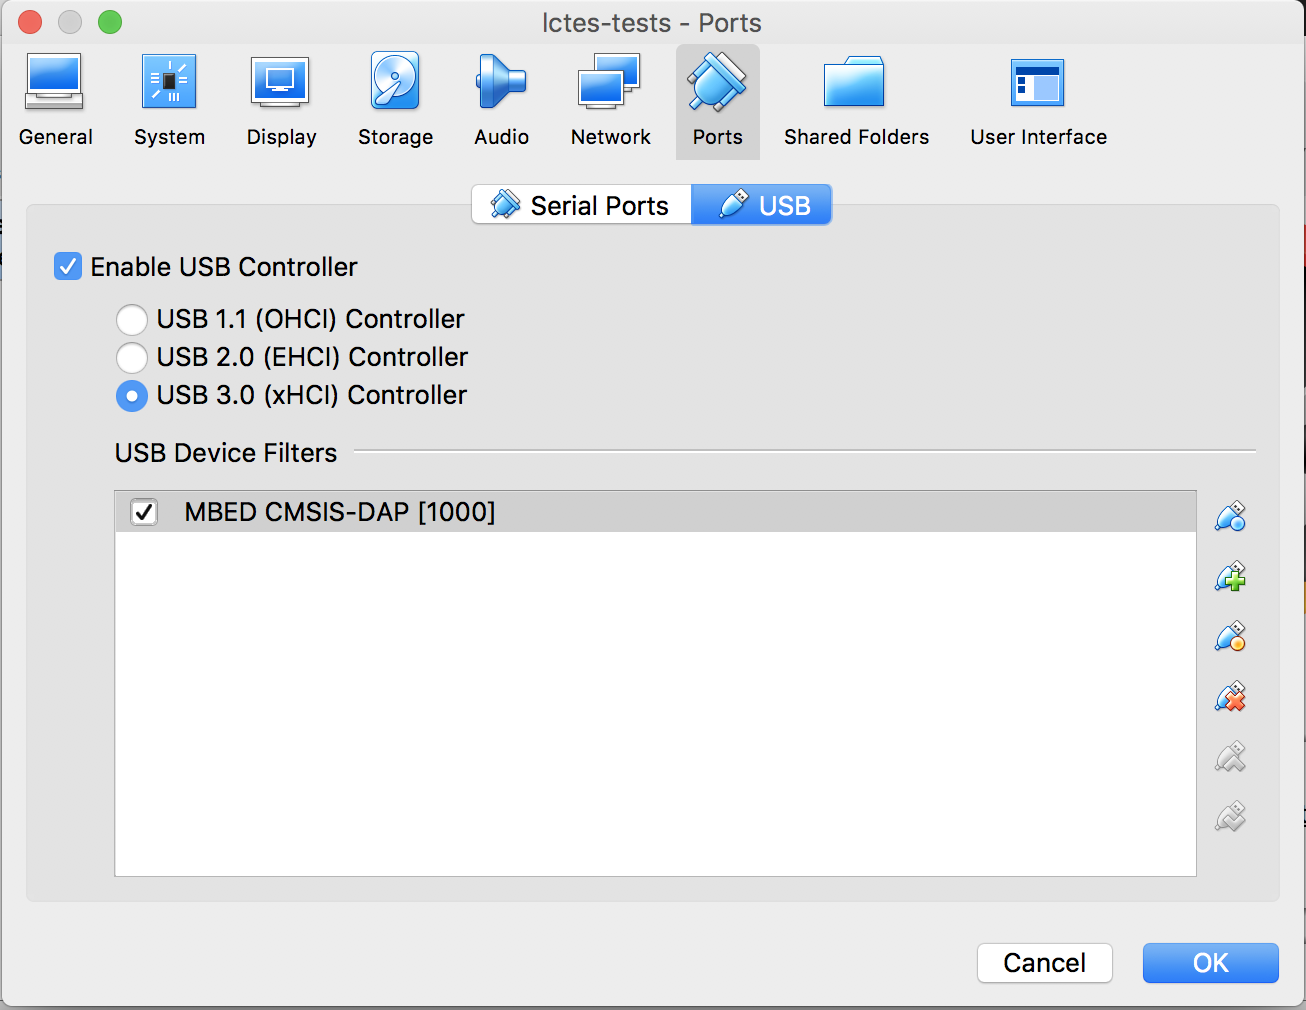
\includegraphics[width=\columnwidth]{images/virtualbox.png}
\end{center}

We also have a convenience script for mounting a shared folder between the host and the vm. Simply create a shared folder named `lctes-vm-dir' and run `sh mount.sh' (contained in evaluators) as a super user to mount the shared folder to vb-share (also contained in evaluators). Shared folder creation in VirtualBox is pictured below:

\begin{center}
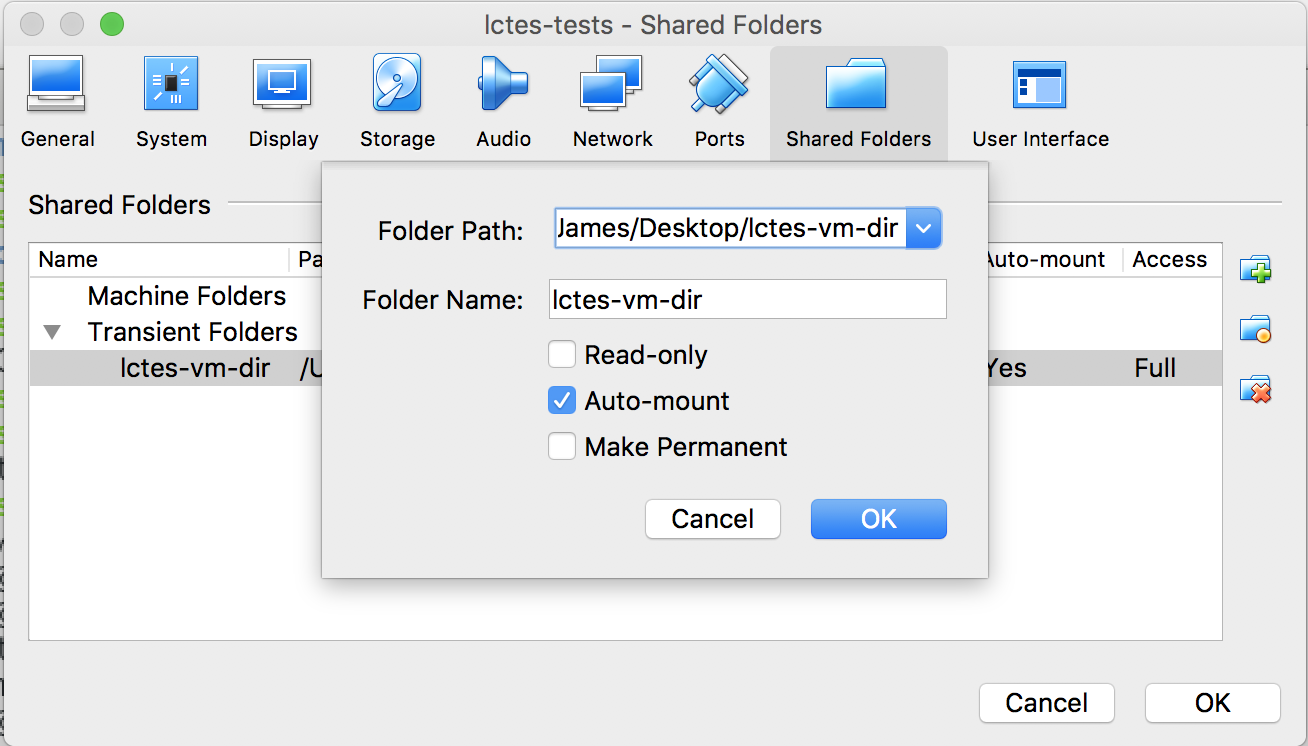
\includegraphics[width=\columnwidth]{images/shared-folder.png}
\end{center}